\subsection*{Problem 8}
\paragraph{}
Here we used 4 different models and their results are shown in Table \ref{table:6}. We noticed some mismatches between the local \textit{movie\_rating.txt} file and data from IMDB top 250 \cite{imdb}. We use IMDB top 250 as the source to provide a list of movies directed by top 100 directors, accounting for the first 166 movies. Out of 100 famous directors, 91 are found in the local \textit{director\_movie.txt} file, with 1069 movies found in \textit{movie\_ratings.txt}.
\paragraph{}
The page rank file contains score for all 113043 actors/actresses. Of the 105595 movies with a population greater than 10, 84485 of them have ratings and we will be focusing on these movies.	
\subsubsection*{Model 1}
\paragraph{}
We start with using top-5 pagerank score only, without extra information from famous director. This is because movies directed by famous directors is accoutable for roughly 1\% of the total data entries. By our experience this director feature would end up with little effects. Therefore for model 1 we used only 5 features.
\subsubsection*{Model 2}
\paragraph{}
For model 2 we added famous director and we simply combined them into 1 column, i.e., if a movie is directed by any of these directors, we assign a value of 1, and 0 otherwise. In the end model 2 used 6 features.
\subsubsection*{Model 3}
\paragraph{}
For model 3 we created another column of director dummy variable, i.e., if a movie is directed by any of these directors, we assign a value of 0, and 1 otherwise. Therefore for model 3 there is a total of 7 features.
\subsubsection*{Model 4}
\paragraph{}
For model 4 we separated these 91 famous director into 91 columns, and combined with top-5 pagerank score, there is a total of 96 features.

\begin{table}[h!]
	\centering
	\caption{Regression Analysis of the 3 Target Movies}
	\begin{tabular}{{|c|}*{4}{|c|}}
		\hline
		&Movie Name 	& Batman v Superman:     & Mission: Impossible & Minions(2015)   	\\
	    &           	& Dawn of Justice(2016)  & Rogue Nation(2015)  &               		\\
		\hline
		&Actual Rating  & 7.1  	                 & 7.5                 & 6.4    			\\ 
		\hline
		&Model1 Rating  & 6.15722109  	          & 6.15722109         & 6.15722109   		\\ 
		\hline
		&Model2 Rating  & 6.17290303  	          & 6.17290303         & 6.17290303   		\\ 
		\hline
		&Model3 Rating  & 6.15751179  	          &  6.15751179        & 6.15751179  		\\ 
		\hline
		&Model4 Rating  & 6.16009448  	          & 6.16009448         & 6.16009448  		\\ 
		\hline
	\end{tabular}
	\label{table:6}
\end{table}

\paragraph{}
All models, as expected, generate similar results and does not provide a very good fit. This is mainly attributable to two factors. First, regression models usually relies on a large number of meaningful features to provide discretion from input to output. Otherwise it result in exactly what we see in Table \ref{table:6}, a homogenization of outputs. And by meaningful it means that features should be as independent as possible. Although in model 4 we had a total of 96 features, 91 of them are all related to director popularity and are highly correlated, which renders them ineffective. Second, the pagerank score are related to, primarily, number of movies involved but not popularity, or quality of the actor/actress, and therefore does not serve as a good indicator whether a movie should be welcomed or not. Table \ref{table:7} presents the fitting performance in average root mean square error (ARMSE), error variance or mean square error (MSE), and mean error. And Figure \ref{fig:pgsample} presents the cross validation score of model 1 (others are similar) as sample size increases. This simply means that the potential of these models are very limited.

\begin{table}[h!]
	\centering
	\caption{Performance of the 4 Models}
	\begin{tabular}{{|c|}*{4}{|c|}}
		\hline
		&            	& ARMSE     			  & Error Variance (MSE)  & Mean Error \\
		\hline
		&Model1   		& 1.194394  	          & 1.430786          	  & 0.112465 \\ 
		\hline
		&Model2   		& 1.194749  	          & 1.427424          	  & 0.120511 \\ 
		\hline
		&Model3  		& 1.263320  	          & 1.595977          	  &	0.081992 \\ 
		\hline
		&Model4 		& 1.188299  	          & 1.412056          	  &	0.114583 \\ 
		\hline
	\end{tabular}
	\label{table:7}
\end{table}

\begin{figure}[h]
	\centering
	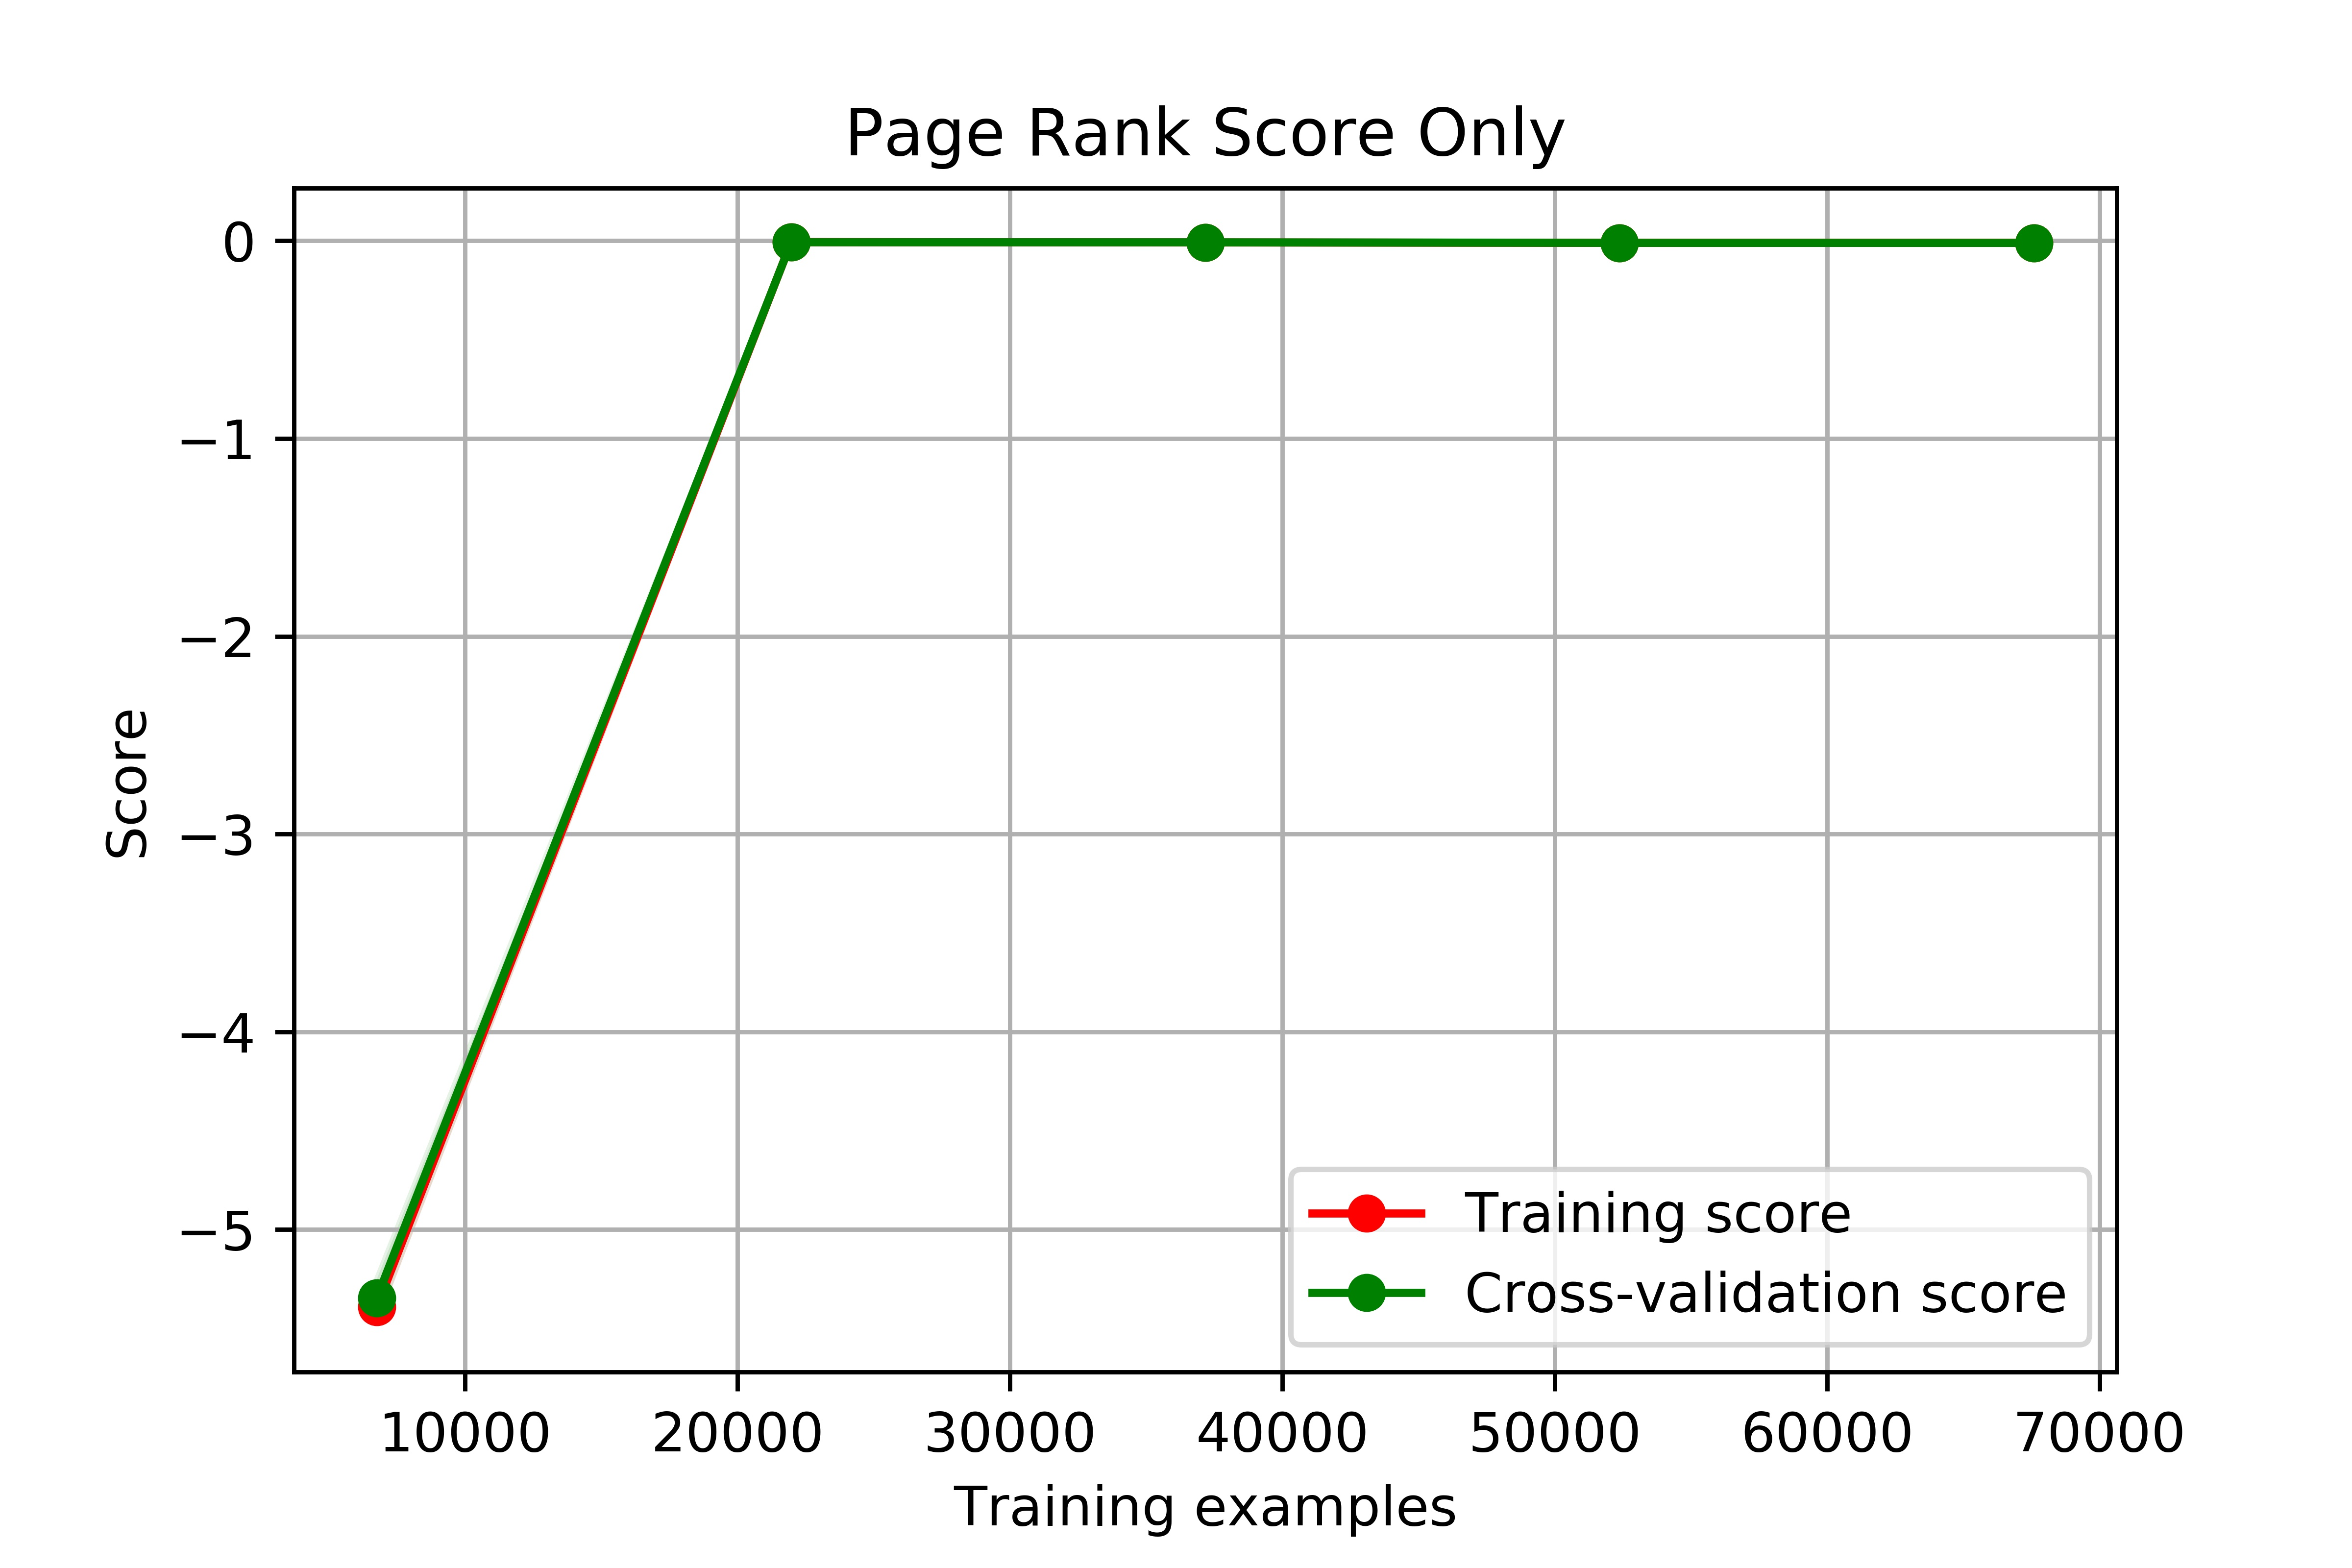
\includegraphics[width=.7\linewidth]{pg01.jpg}
	\caption{Cross Validation Score as Training Size Increases}	
	\label{fig:pgsample} 
\end{figure}